\newpage
\section{User Interface Design}
\subsection{Homepage}
In both mobile application and browser, from homepage it's possible to move to all functions: login, registration, request and reservation (these two only for users registered as passengers) and Manage work (only for users registered as taxi drivers).
\begin{figure}[H]
\centering
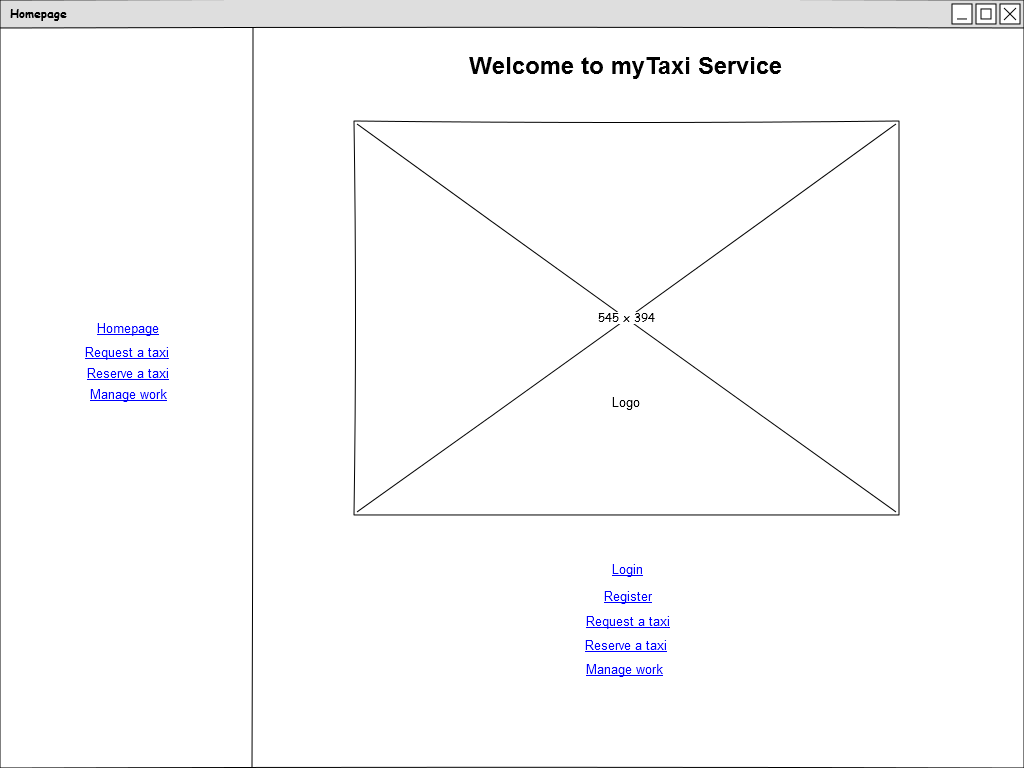
\includegraphics[scale=0.3]{mockups/homepage_web.png}
\caption{Homepage Web Version}
\end{figure}
\begin{figure}[H]
\centering
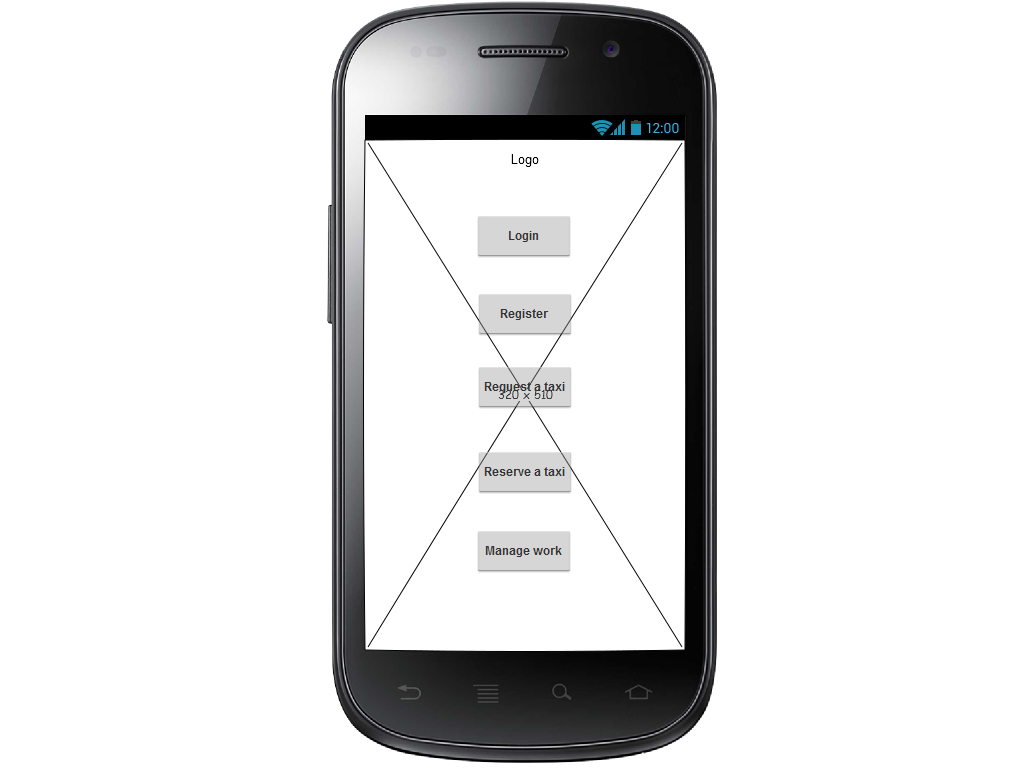
\includegraphics[scale=0.3]{mockups/homepage_mobile.png}
\caption{Homepage Mobile Version}
\end{figure}
\break
\subsection{Registration}
Users can register themselves from this page filling various fields. The majority of these last ones are in common for every person who wants to register, but there is a field reserved to taxi drivers (taxi driver license number) that can be filled only choosing taxi driver, in the web registration page menu, or taxi driver radio in the mobile registration page. \newline Before confirming the registration, it's necessary to accept policies about privacy and use of user's personal details. \newline
From this browser page users can go to homepage and other important pages.
\begin{figure}[H]
\centering
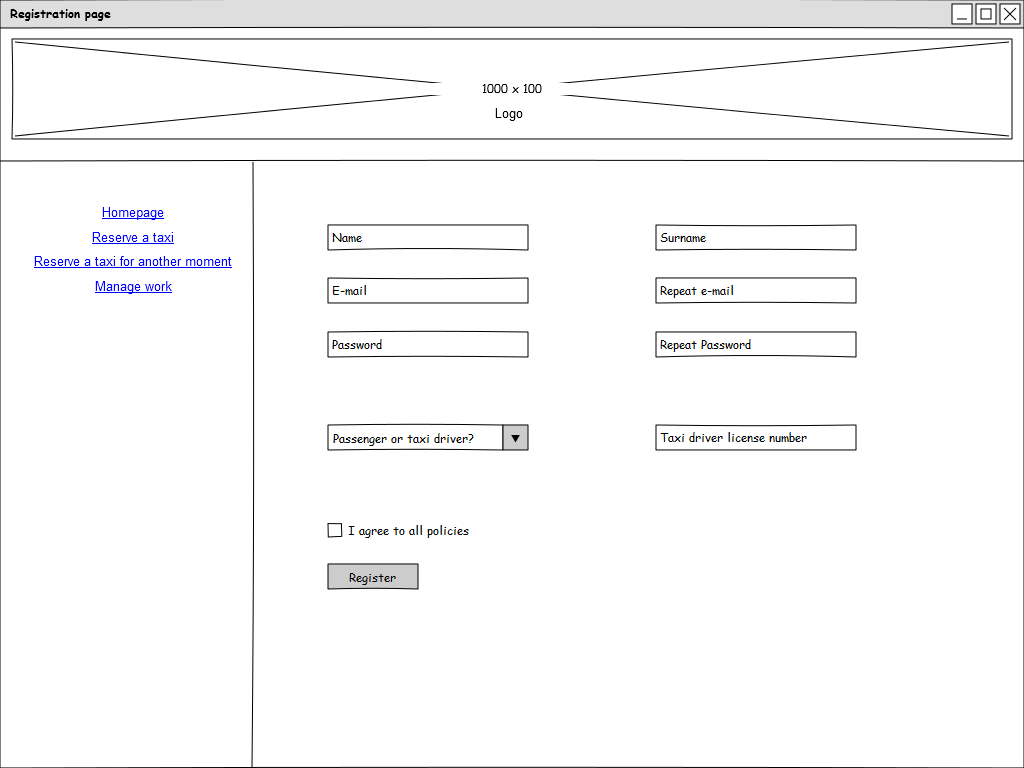
\includegraphics[scale=0.35]{mockups/registration_web.png}
\caption{Registration Web Version}
\end{figure}
\begin{figure}[H]
\centering
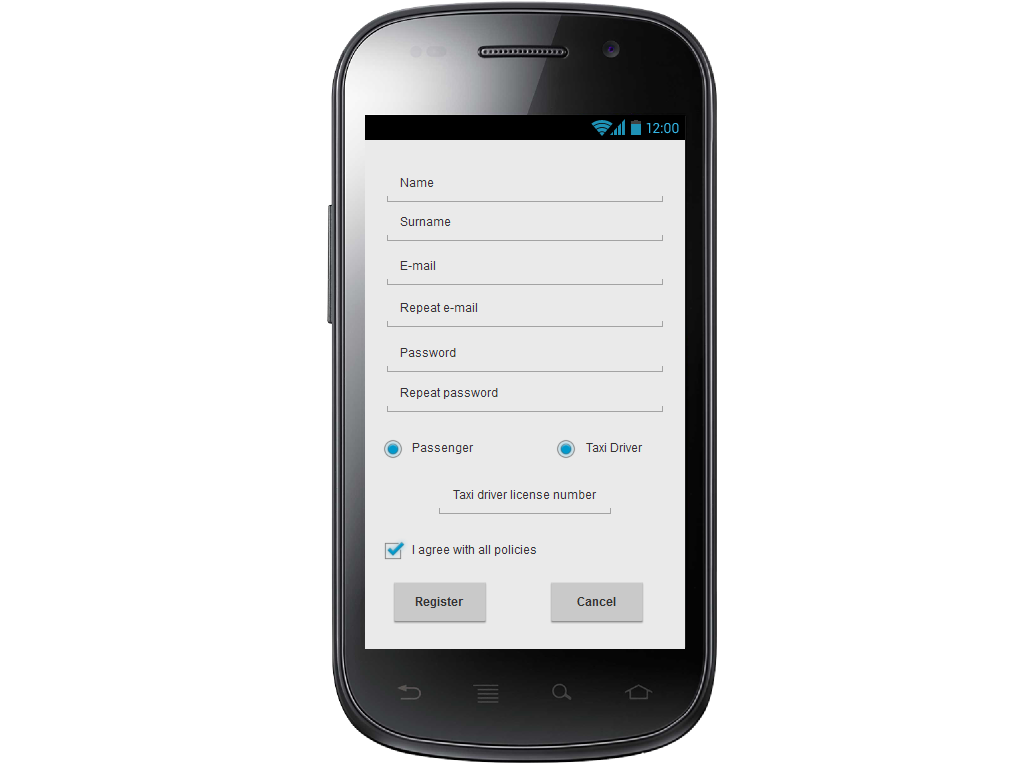
\includegraphics[scale=0.35]{mockups/registration_mobile.png}
\caption{Registration Mobile Version}
\end{figure}
\break
\subsection{Login}
From this page registered users can log in inserting either the registration email or username and the password chosen during registration. \newline If an user forgets his/her password, username or email, it's possible to recover them: a message on the mobile phone or an email is sent to him/her. \newline Also from this browser page users can go to homepage and other important pages.
\begin{figure}[H]
\centering
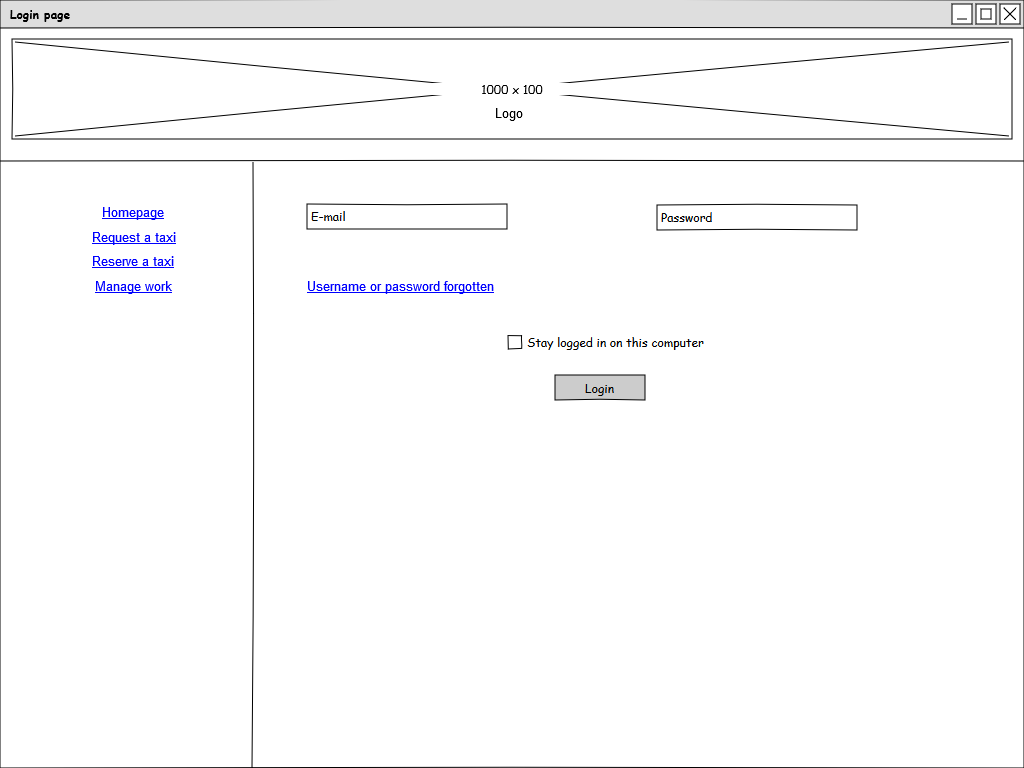
\includegraphics[scale=0.35]{mockups/login_web.png}
\caption{Login Web Version}
\end{figure}
\begin{figure}[H]
\centering
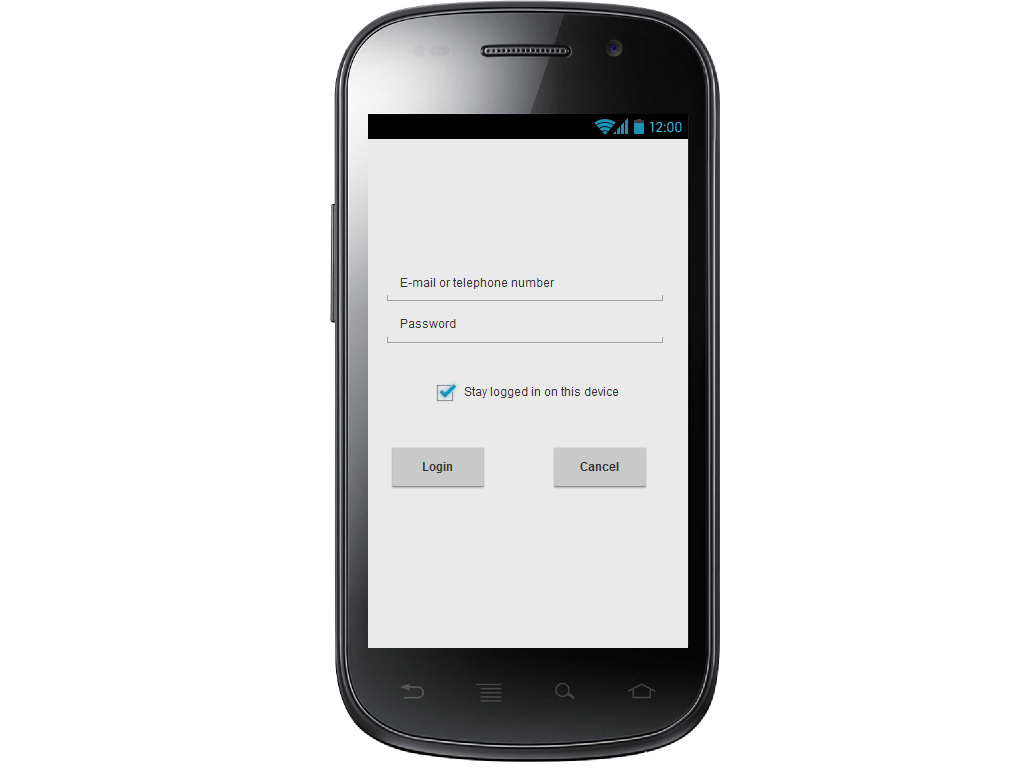
\includegraphics[scale=0.35]{mockups/login_mobile.png}
\caption{Login Mobile Version}
\end{figure}
\break
\subsection{Request}
The mockups below shows the page in which a Registered Passenger can make a request
\begin{figure}[H]
\centering
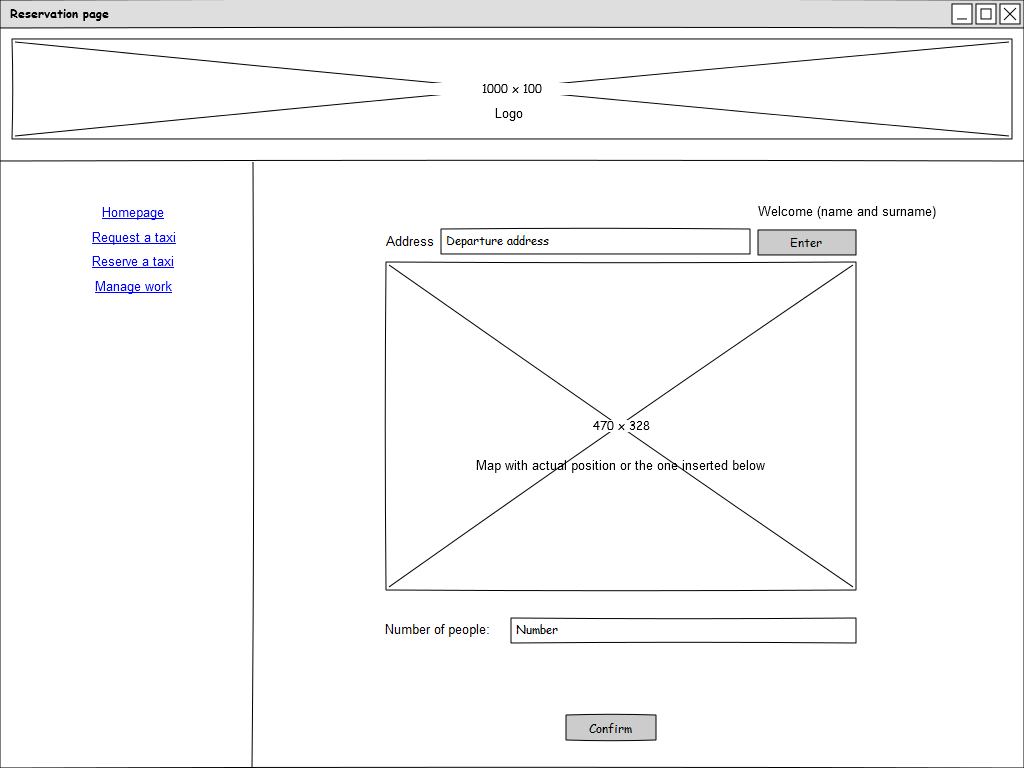
\includegraphics[scale=0.35]{mockups/request_web.png}
\caption{Request Web Version}
\end{figure}
\begin{figure}[H]
\centering
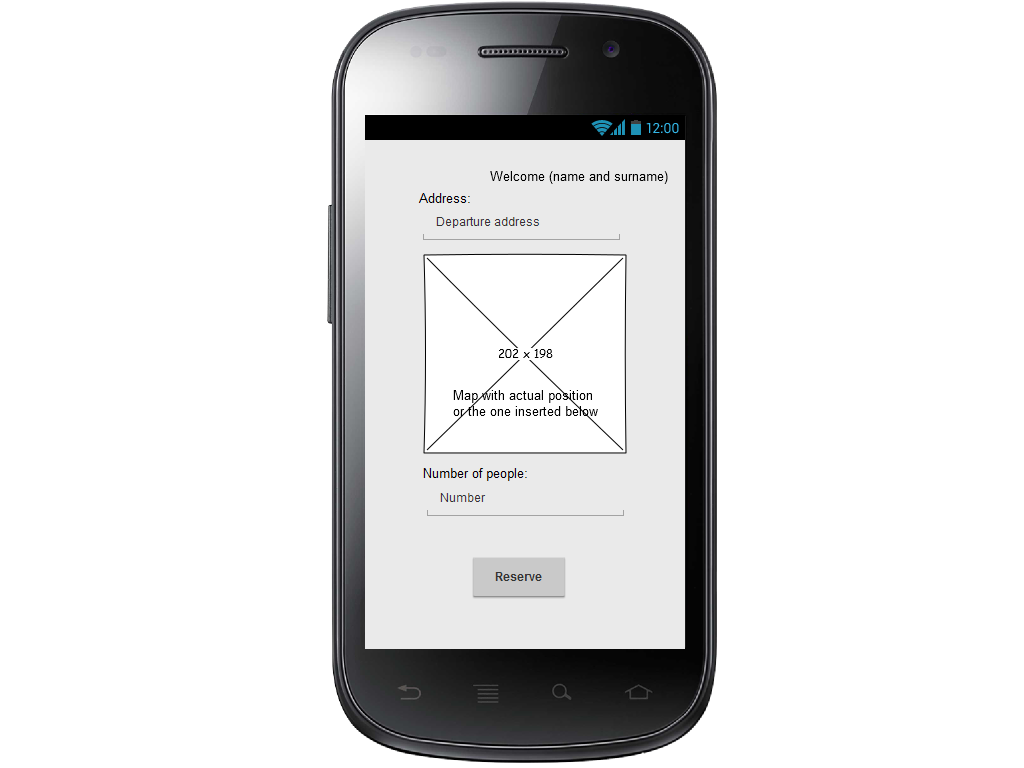
\includegraphics[scale=0.35]{mockups/request_mobile.png}
\caption{Request Mobile Version}
\end{figure}
\break
\subsection{Reservation}
The mockups below shows the page in which a Registered Passenger can make a reservation
\begin{figure}[H]
\centering
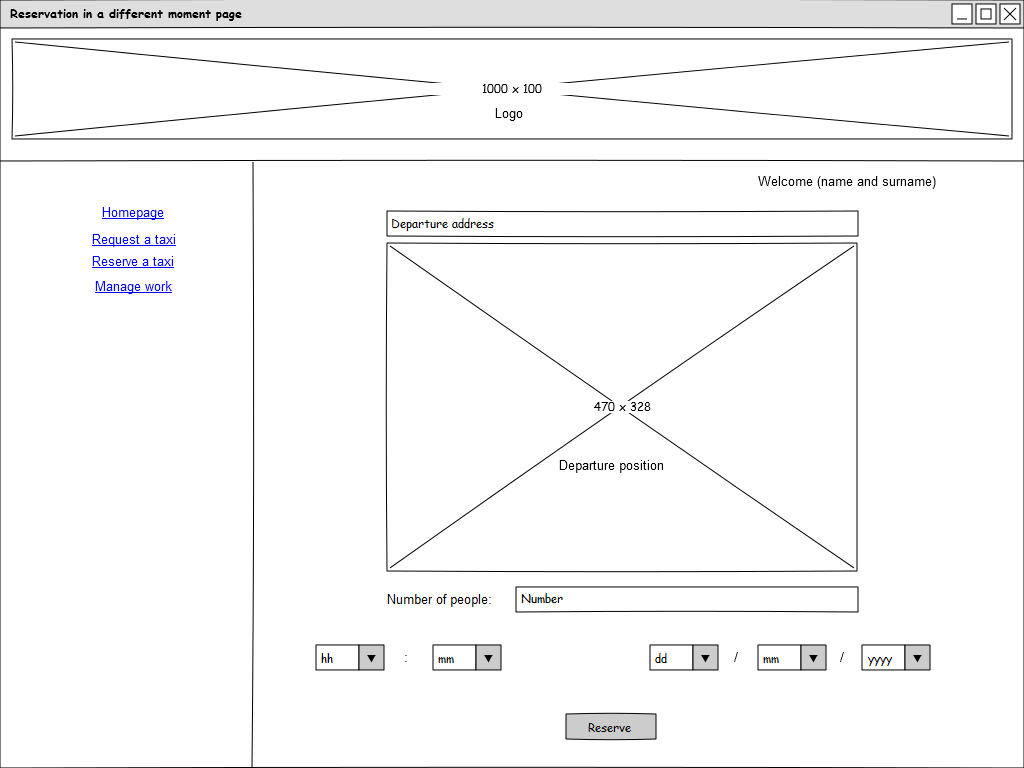
\includegraphics[scale=0.35]{mockups/reservation_web.png}
\caption{Reservation Web Version}
\end{figure}
\begin{figure}[H]
\centering
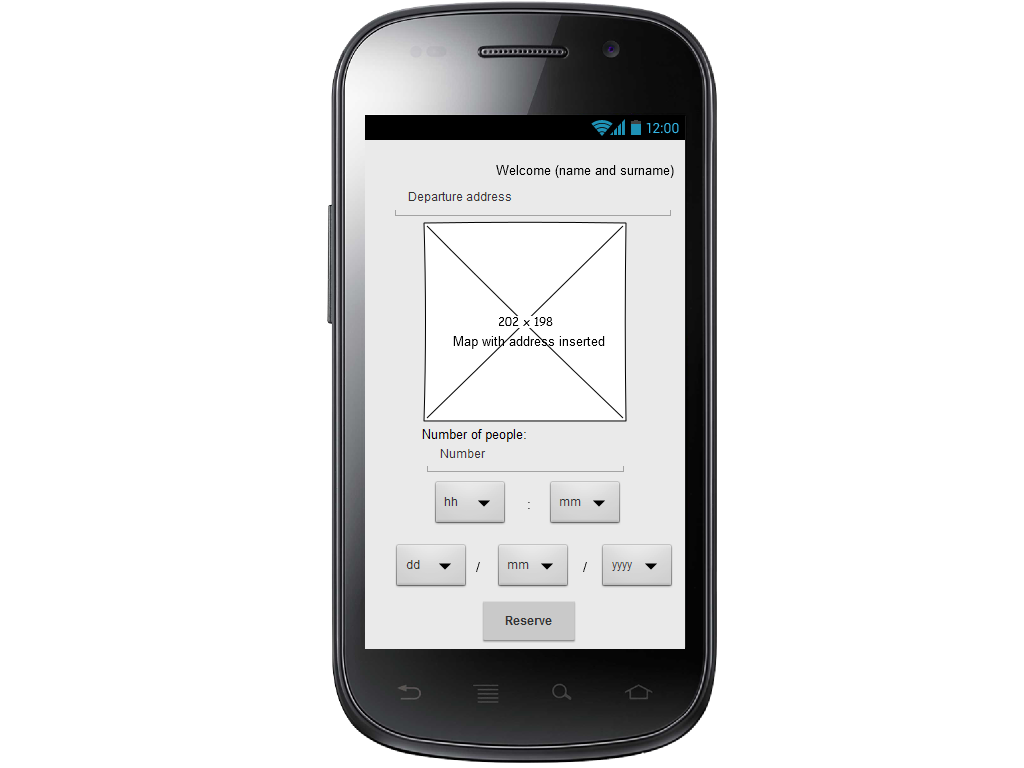
\includegraphics[scale=0.35]{mockups/reservation_mobile.png}
\caption{Reservation Mobile Version}
\end{figure}
\break
\subsection{Driver Interface}
The mockups below shows the page in which a Driver can manage an incoming request
\begin{figure}[H]
\centering
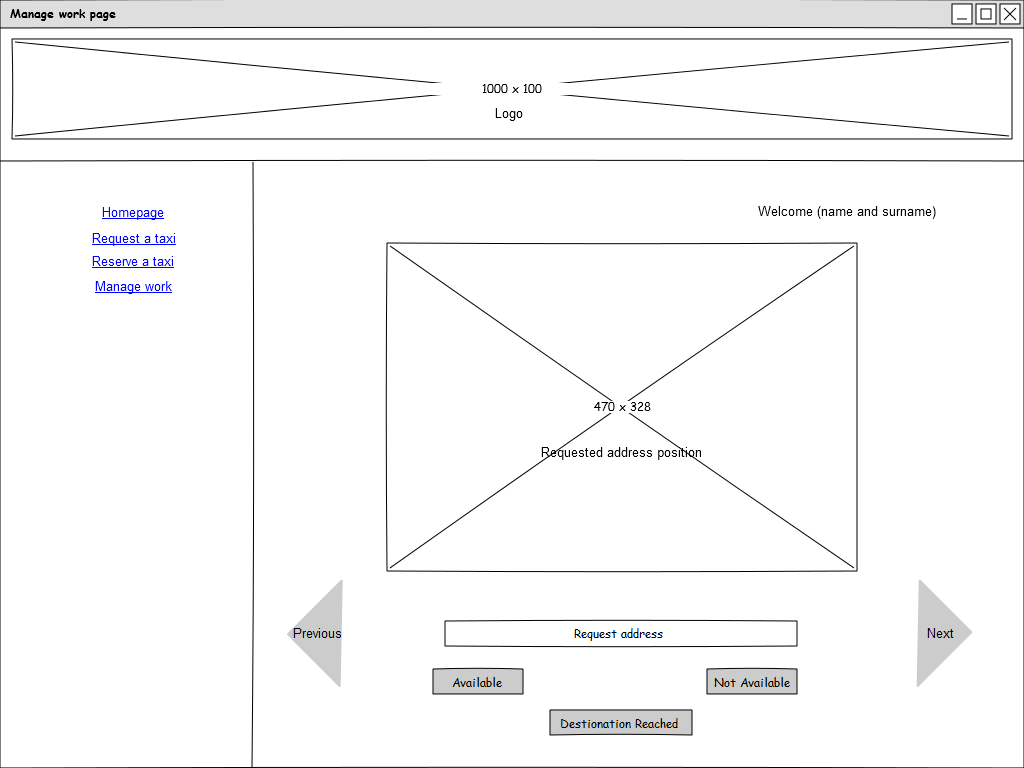
\includegraphics[scale=0.35]{mockups/manage_work_web.png}
\caption{Driver Interface Web Version}
\end{figure}
\begin{figure}[H]
\centering
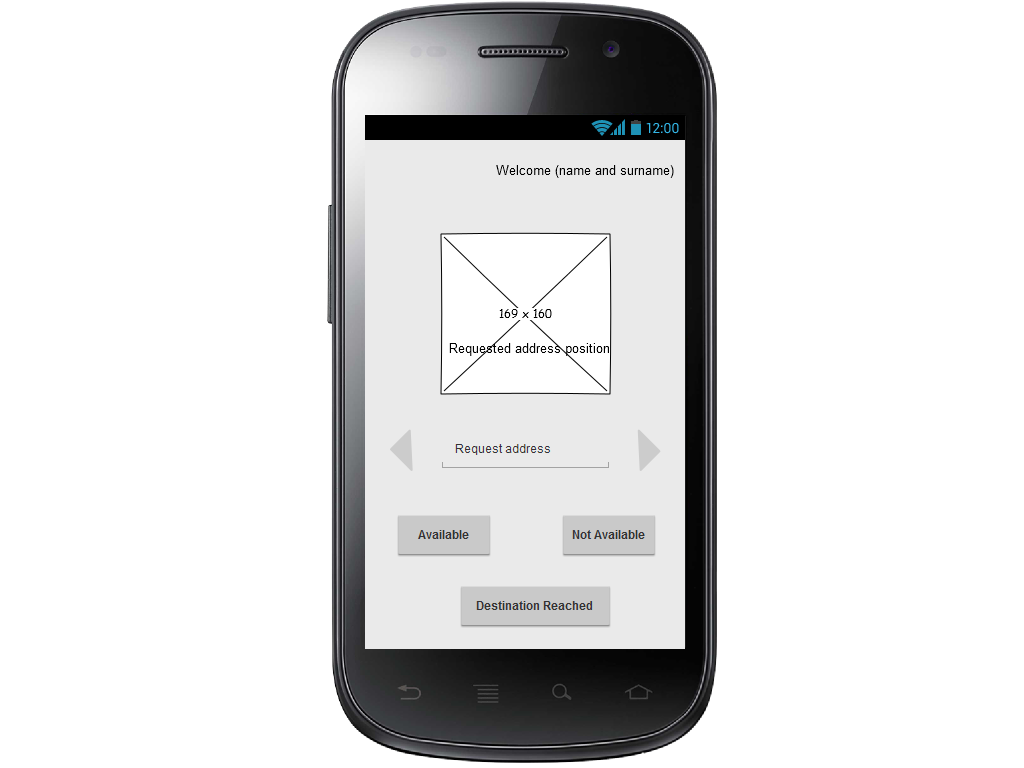
\includegraphics[scale=0.35]{mockups/manage_work_mobile.png}
\caption{Driver Interface Mobile Version}
\end{figure}
\break